\begin{frame}
	\frametitle{猫群算法概述}
	猫群算法(Cat Swarm Optimization,缩写为CSO)是由Shu-An Chu等人在2006 年首次提出来的一种基于猫的行为的全局优化算法。根据 生物学分类,猫科动物大约有 32 种,例如: 狮子、老虎 、豹子 、猫等。尽管生存环境不同 ,但是猫科动物的很多生活习性非常相似。猫的警觉性非常高,即使在休息的时候也处于一种高度的警惕状 态,时刻保持对周围环境的警戒搜寻; 它们对于活动的目标具有强烈的好奇心,一旦发现目标便进行跟踪,并且能够迅速地捕获到猎物。猫群算法正是关注了猫的搜寻和跟踪两种行为。
\end{frame}


\begin{frame}
	\frametitle{猫群算法概述}
	猫群算法中,猫即待求优化问题的可行解。猫群算法将猫的行为分为两种模式,一种就是猫在懒散、环顾四周状态时的模式称之为搜寻模式; 另一种是在跟踪动态目标时的状态称之为跟踪模式。猫群算法中,一部分猫执行搜寻模式,剩下的则执行跟踪模式,两种模式通过结合率 MR( Mix- ture Ratio) 进行交互,MR 表示执行跟踪模式下的猫的数量在整个猫群中所占的比例,在程序中 MR 应为一个较小的值。利用猫群算法解决优化问题,首先需要确定参与优化计算的个体数,即猫的数量。每只猫的属性( 包括由 M 维组成的自身位 置) 、每一维的速度、对基准函数的适应值及表示猫是处于搜寻模式或者跟踪模式的标识值。当猫进行完搜寻模式和跟踪模式后,根据适应度函数计算它们的适应度并保留当前群体中最好的解。之后再根据结合率随机地将猫群分为搜寻部分和跟踪部分的猫,以此方法进行迭代计算直到达到预设的迭代次数。
\end{frame}


\begin{frame}
	\frametitle{猫群算法概述}
	\begin{columns}
	\column{.7\textwidth}
		\begin{itemize}
			\item {数学描述}
				\begin{itemize}
					\item {搜寻模式用来模拟猫的当前状态,分别为休息、四处查看、搜寻下一个移动位置。在搜寻模式中,定义了 4 个基本要素: 记忆池(SMP)、变化域 (SRD)、变化数(CDC)、自身位置判断(SPC)。SMP 定义了每一只猫的搜寻记忆大小,表示猫所搜寻到的位置点,猫将根据适应度大小从记忆池中选择一个最好的位置点。SRD表示选择域的变异率,搜寻模式中,每一维的改变范围由变化域决定,根据经验一般取值为 0.2。CDC 指每一只猫将要变异的维数的个数,其值是一个从 0 到总维数之间的随机值。SPC是一个布尔值,表示猫是否将已经过的位置作为将要移动到的候选位置之一,其值不影响 SMP 的取值。}		
				\end{itemize}
		\end{itemize}
	\column{.4\textwidth}
		\begin{figure}[p]
			\centering
			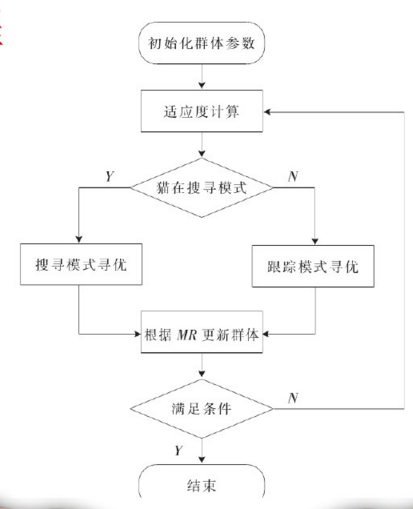
\includegraphics[width=6cm]{pic/cat4.png}
			\caption{流程图}
		\end{figure}
	\end{columns}
\end{frame}

\begin{frame}
	\frametitle{猫群算法概述}
	\begin{columns}
	\column{.6\textwidth}
		\begin{itemize}
			\item {搜寻模式过程描述}
				\begin{itemize}
					\item {将当前位置复制j份副本放在记忆池中,j = SMP,即记忆池的大小为 j; 如果 SPC 的值为真, 令 j = ( SMP - 1) ,将当前位置保留为候选解。}
					\item {对记忆池中的每个个体副本,根据 CDC 的大小,随机地对当前值加上或者减去SRD\%(变化域由百分率表示),并用更新后的值来代替原来的值}
					\item {分别计算记忆池中所有候选解的适应度值。}
					\item {从记忆池中选择适应度值最高的候选点来代替当前猫的位置,完成猫的位置更新。}	
				\end{itemize}
		\end{itemize}
	\column{.4\textwidth}
		\begin{figure}[htbp]
			\centering
			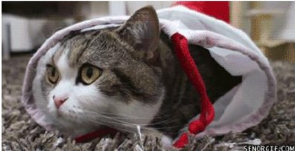
\includegraphics[width=6cm]{pic/cat1.png}
			\caption{搜寻模式}
		\end{figure}
	\end{columns}
\end{frame}

\begin{frame}
	\frametitle{猫群算法概述}
	\begin{columns}
	\column{.7\textwidth}
		\begin{itemize}
			\item {跟踪模式过程描述}
				\begin{itemize}
					\item {速度更新。整个猫群经历过的最好位置, 即目前搜索到的最优解,记做 $X_{best}$ 。每只猫的速度记做$v_i ={v_{i1},v_{i2},...,v_{id}}$,每只猫根据公式(1) 来更新自己的速度。$$v_{i,d}(t+1) = v^{i,d}(t) + r^* c^*(X_{best,d}(t) - x_{i,d}(t)),d = 1,2,…M (1) $$ 
$v_{i,d}(t+1)$表示更新后第 i 只猫在第 d 维的速度值,M 为维数大小; 
$X_{best,d}(t)$ 表示猫群中当前具有最好适应度值的猫的位置; 
$x_{i,d}(t)$ 指当前第 i 只 猫在第 d 维的位置,\\c 是个常量,其值需要根据不同的问题而定。
r 是一个[0,1]之间的随机值。}
					\item {判断每一维的速度变化是否都在SRD内。给每一维的变异加一个限制范围,是为了防止其变化过大,造成算法在解空间的盲目随机搜索。SRD在算法执行之前给定,如果每一维改变后的值超出了SRD的限制范围,则将其设定为给定的边界值。}
				\end{itemize}
		\end{itemize}
	\column{.4\textwidth}
		\begin{figure}[htbp]
			\centering
			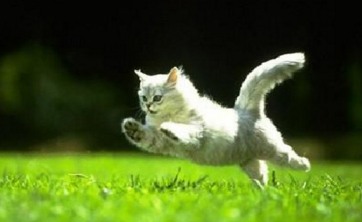
\includegraphics[width=6cm]{pic/cat3.png}
			\caption{跟踪模式}
		\end{figure}
	\end{columns}
\end{frame}

\begin{frame}
	\frametitle{猫群算法概述}
	\begin{columns}
	\column{.7\textwidth}
		\begin{itemize}
			\item {跟踪模式过程描述}
				\begin{itemize}
					\item {位置更新。根据公式(2)利用更新后的速度来更新猫的位置。$$x_{i,d}(t+1) = x_{i,d}(t) + v_{i,d}(t+1), (2) d = 1,2,…M$$ 试中$x_i(t+1)$表示第i只猫更新后的位置。}
				\end{itemize}
		\end{itemize}
	\column{.4\textwidth}
		\begin{figure}[htbp]
			\centering
			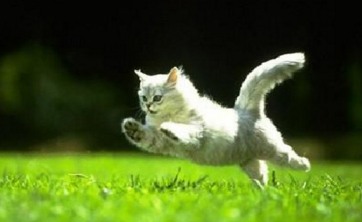
\includegraphics[width=6cm]{pic/cat3.png}
			\caption{跟踪模式}
		\end{figure}
	\end{columns}
\end{frame}
\begin{frame}
	\frametitle{算法改进研究}
		\begin{itemize}
					\item {Santosa Budi 等( 2009 年)提出一种基于聚类问题的猫群算法,对猫群优化公式进行修正,提高了猫群算法优化聚类问题的优化性能。Yong - Guo Liu 等( 2010 年)引入最新的元启发式方法到猫群算法中,用以寻找最优的数据集聚类方法。}
					\item {引入K - Harmonic 均值操作改善种群并促进 聚类算法的收敛,提出了 2 种基于猫群算法的聚类方法,分别为猫群优化聚类法、K - harmonic 均值猫群优化聚类法。}
					\item {范凯波(2011年)通过研究群体智能计算,提出了基于猫群算法优化的 k-均值聚类算法,实现了车辆目标的分类。}
					\item {Orouskhani Maysam 等(2011年)为提高猫群算法的收敛性,在位置更新方程内增加一个新的参数作为惯性加权,在算法的追踪模型中使用新的速率更新方程,提出一种加权平均惯性猫群算法。}
			
		\end{itemize}

\end{frame}

\begin{frame}
	\frametitle{算法应用研究}
		\begin{itemize}
					\item {王光彪等( 2011 年)针对传统进化算法在图像分类中存在的收敛速度慢、易陷入局部最优等问题,提出用猫群算法求解图像分类问题,将求解组合优化问题转化为猫群的位置寻优过程,并 分析了猫群算法及其两种行为模式下的算法模型。验证了猫群算法在图像分类中的准确性和有效性。}
					\item {Zhi-HuiWang等(2012年)针对最低有效位替换方法解决隐秘图像问题时运行时间长的问 题,通过改进猫群优化策略来获取解决隐秘图像 质量问题的最优解或次优解。}
					\item {Long Xu 等( 2012 年)针对资源受限项目调度问题提出一种基于猫群算法的方法。通过猫的多维位置提供解决资源受限项目调度问题的潜在方案,包括 3 个步骤: 先随机初始化猫的参数,然后迭代位置,通过串行 SGS 方法计算适应度,最后如果条件满足则终止程序。}
					\item {Shi - Yu Cui 等( 2013 年) 针对原始块截断编码方法的复杂性难以找到有效的常用点阵图,利用猫群算法进行块截断编码,提出一种基于此种编码方式的图像压缩技术。}
		
		\end{itemize}

\end{frame}

\begin{frame}
	\frametitle{总结}
	猫群算法的研究刚刚起步,一些思想处于萌芽阶段,严格的理论基础尚不成熟。对于算法本身的思想、原理、参数设置以及种群多样性的研究,仍停留在实验探索阶段,并未有更深入的分析与讨论。关于算法收敛性的分析与证明的研究还未出现。对猫群算法的改进技术主要集中于常态的增加参数、加入部分操作算子等方面,对于算法框架、迭代进化方式等的改进的研究较少。部分学者将粒子群算法以及混沌搜索等算法 或思想引入猫群算法,在一定程度上提高了算法的优化性能,但仍然存在易陷入“早熟”、运行速度 慢等缺陷,并且,被引入算法仅执行猫群算法的单个行为。

\end{frame}